\input{includes/lab_preamble}
\usepackage{tikz}
\usetikzlibrary{matrix, positioning}

\def\LabCourse{AP Computer Science A}
\def\LabNumber{03}
\def\LabTitle{Cellular Automata}

\newcommand\QBlankBox[1]{
\stepcounter{QuestionCounter}
\colorbox{black!10}{\parbox{0.9875\textwidth}{
  \raggedright
  \textbf{Question \#\theQuestionCounter:} #1
}}
}

\begin{document}
	\begin{coverpages}
		\ \\[2cm]
		\begin{center}
			\huge
			\textbf{\LabTitle}

			\Large
			\LabCourse
		\end{center}

		\vspace{1.5cm}

		\begin{center}
			\includegraphics[scale=0.45]{graphics/logo_black}

			\vspace{2.5cm}

			\Large
			Name: \rule{11.5cm}{0.1pt}
		\end{center}
	\end{coverpages}

	\thispagestyle{empty}
	\tableofcontents

	\pagebreak

	\section{Background}
		\begin{center}
	    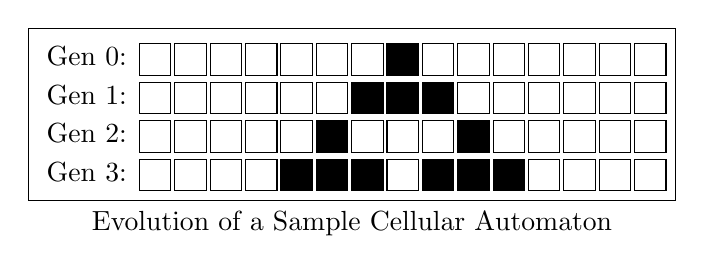
\begin{tikzpicture}[b/.style={draw, minimum size=4mm, fill=black},w/.style={draw, minimum size=4mm},m/.style={matrix of nodes, column sep=1pt, row sep=0pt, draw}, node distance=1pt]
	      \matrix [m,label=below:Evolution of a Sample Cellular Automaton]{
	        \node[anchor=mid]{Gen 0:}; &|[w]|&|[w]|&|[w]|&|[w]|&|[w]|&|[w]|&|[w]|&|[b]|&|[w]|&|[w]|&|[w]|&|[w]|&|[w]|&|[w]|&|[w]|\\
	        \node[anchor=mid]{Gen 1:}; &|[w]|&|[w]|&|[w]|&|[w]|&|[w]|&|[w]|&|[b]|&|[b]|&|[b]|&|[w]|&|[w]|&|[w]|&|[w]|&|[w]|&|[w]|\\
	        \node[anchor=mid]{Gen 2:}; &|[w]|&|[w]|&|[w]|&|[w]|&|[w]|&|[b]|&|[w]|&|[w]|&|[w]|&|[b]|&|[w]|&|[w]|&|[w]|&|[w]|&|[w]|\\
	        \node[anchor=mid]{Gen 3:}; &|[w]|&|[w]|&|[w]|&|[w]|&|[b]|&|[b]|&|[b]|&|[w]|&|[b]|&|[b]|&|[b]|&|[w]|&|[w]|&|[w]|&|[w]|\\
	      };
	    \end{tikzpicture}
	  \end{center}

	  The above image is of the first few generations of an \emph{elementary cellular automaton}, a concept discussed at length in Stephen Wolfram's massive work: \emph{A New Kind of Science}. In this text, Wolfram continues the work first started in the 1940's, when Stanislaw Ulam and John von Neumann suggested the use of cellular automata for a number of different, important areas of research having to do with replication of various different natural and technological systems (von Neumann, in particular, was interested in self-replicating robots).\\[\baselineskip]
	  A cellular automaton attempts to represent these systems as a grid of cells, each of which is in a specific current state. These cells will evolve based on the states of cells in their \emph{neighborhood}, an important concept that will be discussed at length shortly. Once these cells have evolved, the entire set of cells enters a new state, called a \emph{generation} of the cellular automaton.\\[\baselineskip]
	  Although Wolfram's assertation that the study of these ``cellular automata'' are relevant for all branches of science can be controversial, their academic interest within the computer sciences is fairly undisputed. In this lab, we will be looking at the concept of \emph{elementary cellular automata}, a set of cellular automatons based on a single-dimensional array of cells that evolve according to a number of preset rules.

		\subsection{Elementary Cellular Automata}
		  An elementary cellular automaton is a single-dimensional array of cells, each of which can be in one of two states ($0$ and $1$ or ``off'' and ``on'', however you'd like to think of it). A neighborhood for each cell is comprised of three cells: the cell itself, and the cells on either side of it (left and right). Additionally, the starting state (often referred to as ``generation zero'') has all cells in the same state, except for the very center cell. A visualisation of the starting state for every elementary cellular automaton is below.

		  \begin{center}
		    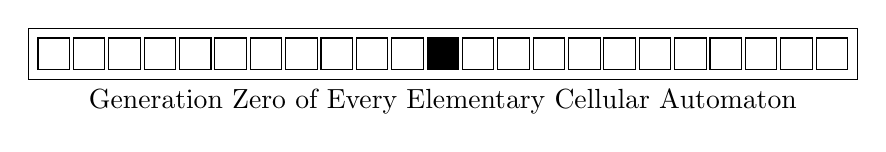
\begin{tikzpicture}[b/.style={draw, minimum size=4mm, fill=black},w/.style={draw, minimum size=4mm},m/.style={matrix of nodes, column sep=1pt, row sep=0pt, draw}, node distance=1pt]
		      \matrix [m,label=below:Generation Zero of Every Elementary Cellular Automaton]{
		         |[w]|&|[w]|&|[w]|&|[w]|&|[w]|&|[w]|&|[w]|&|[w]|&|[w]|&|[w]|&|[w]|&|[b]|&|[w]|&|[w]|&|[w]|&|[w]|&|[w]|&|[w]|&|[w]|&|[w]|&|[w]|&|[w]|&|[w]|\\
		      };
		    \end{tikzpicture}
		  \end{center}

		  Since each neighbourhood contains three cells, there are $8$ possible permutations of neighbourhoods. Note that because the cells on either edge of the grid would only have two cells in their neighbourhood, a choice needs to be made as to what pattern to match. In the examples found within Wolfram's work, the missing neighbour is treated as a $0$ or `off'. Unless specified otherwise, you should continue this convention for your work on cellular automata. All $8$ permutations (in the order Stephen Wolfram used) are seen below.

		  \begin{center}
		    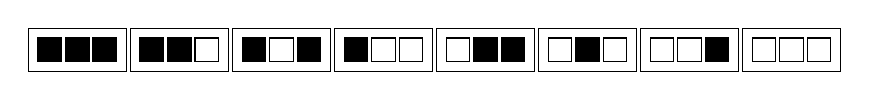
\begin{tikzpicture}[b/.style={draw, minimum size=3mm, fill=black},w/.style={draw, minimum size=3mm},m/.style={matrix of nodes, column sep=1pt, row sep=1pt, draw}, node distance=1pt]
		      \matrix (A) [m]{
		        |[b]|&|[b]|&|[b]|\\
		      };
		      \matrix (B) [m, right=of A]{
		        |[b]|&|[b]|&|[w]|\\
		      };
		      \matrix (C) [m, right=of B]{
		        |[b]|&|[w]|&|[b]|\\
		      };
		      \matrix (D) [m, right=of C]{
		        |[b]|&|[w]|&|[w]|\\
		      };
		      \matrix (E) [m, right=of D]{
		        |[w]|&|[b]|&|[b]|\\
		      };
		      \matrix (F) [m, right=of E]{
		        |[w]|&|[b]|&|[w]|\\
		      };
		      \matrix (G) [m, right=of F]{
		        |[w]|&|[w]|&|[b]|\\
		      };
		      \matrix (H) [m, right=of G]{
		        |[w]|&|[w]|&|[w]|\\
		      };
		    \end{tikzpicture}
		  \end{center}

		  By assigning a result to each of these as either a $0$ or a $1$, we can create a set of rules for each elementary cellular automaton. The following is the set of rules that produced the sample generations above. The block below each neighbourhood represents the state of the cell in the next generation.

		  \begin{center}
		    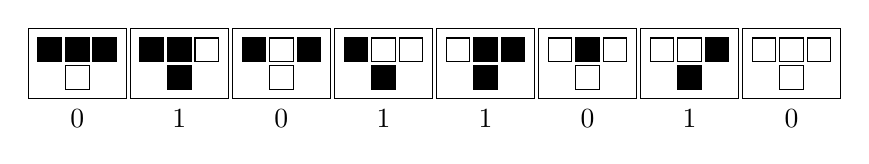
\begin{tikzpicture}[b/.style={draw, minimum size=3mm, fill=black},w/.style={draw, minimum size=3mm},m/.style={matrix of nodes, column sep=1pt, row sep=1pt, draw, label=below:#1}, node distance=1pt]
		      \matrix (A) [m=0]{
		        |[b]|&|[b]|&|[b]|\\
		        &|[w]|\\
		      };
		      \matrix (B) [m=1, right=of A]{
		        |[b]|&|[b]|&|[w]|\\
		        &|[b]|\\
		      };
		      \matrix (C) [m=0, right=of B]{
		        |[b]|&|[w]|&|[b]|\\
		        &|[w]|\\
		      };
		      \matrix (D) [m=1, right=of C]{
		        |[b]|&|[w]|&|[w]|\\
		        &|[b]|\\
		      };
		      \matrix (E) [m=1, right=of D]{
		        |[w]|&|[b]|&|[b]|\\
		        &|[b]|\\
		      };
		      \matrix (F) [m=0, right=of E]{
		        |[w]|&|[b]|&|[w]|\\
		        &|[w]|\\
		      };
		      \matrix (G) [m=1, right=of F]{
		        |[w]|&|[w]|&|[b]|\\
		        &|[b]|\\
		      };
		      \matrix (H) [m=0, right=of G]{
		        |[w]|&|[w]|&|[w]|\\
		        &|[w]|\\
		      };
		    \end{tikzpicture}
		  \end{center}

		  Because the binary string, `01011010', is equivalent to the denary value $90$, the above is referred to as `Rule \#90'. In this way, each ruleset for an elementary cellular automaton can be described by its denary equivalent, with a maximum value of $2^{8} - 1 = 255$.

	\pagebreak

	\section{Applications}
		\QBlankBox{For each of the following rule numbers, write in the appropriate binary digits. Shade each resulting cell, as necessary.}
	    \ \\[9pt]
	    \begin{minipage}{0.25\textwidth}
	      Rule \#62
	    \end{minipage}
	    \begin{minipage}{0.75\textwidth}
	      \begin{center}
	        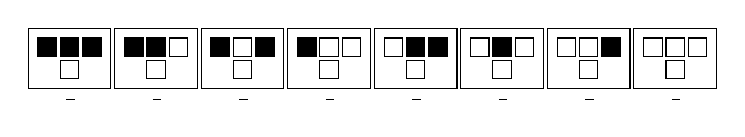
\begin{tikzpicture}[b/.style={draw, minimum size=2mm, fill=black},w/.style={draw, minimum size=2mm},m/.style={matrix of nodes, column sep=1pt, row sep=1pt, draw, label=below:#1}, node distance=1pt]
	          \matrix (A) [m=\_]{
	            |[b]|&|[b]|&|[b]|\\
	            &|[w]|\\
	          };
	          \matrix (B) [m=\_, right=of A]{
	            |[b]|&|[b]|&|[w]|\\
	            &|[w]|\\
	          };
	          \matrix (C) [m=\_, right=of B]{
	            |[b]|&|[w]|&|[b]|\\
	            &|[w]|\\
	          };
	          \matrix (D) [m=\_, right=of C]{
	            |[b]|&|[w]|&|[w]|\\
	            &|[w]|\\
	          };
	          \matrix (E) [m=\_, right=of D]{
	            |[w]|&|[b]|&|[b]|\\
	            &|[w]|\\
	          };
	          \matrix (F) [m=\_, right=of E]{
	            |[w]|&|[b]|&|[w]|\\
	            &|[w]|\\
	          };
	          \matrix (G) [m=\_, right=of F]{
	            |[w]|&|[w]|&|[b]|\\
	            &|[w]|\\
	          };
	          \matrix (H) [m=\_, right=of G]{
	            |[w]|&|[w]|&|[w]|\\
	            &|[w]|\\
	          };
	        \end{tikzpicture}
	      \end{center}
	    \end{minipage}
	    \ \\[27pt]
	    \begin{minipage}{0.25\textwidth}
	      Rule \#108
	    \end{minipage}
	    \begin{minipage}{0.75\textwidth}
	      \begin{center}
	        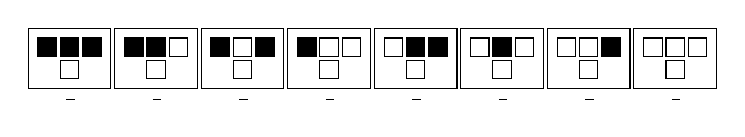
\begin{tikzpicture}[b/.style={draw, minimum size=2mm, fill=black},w/.style={draw, minimum size=2mm},m/.style={matrix of nodes, column sep=1pt, row sep=1pt, draw, label=below:#1}, node distance=1pt]
	          \matrix (A) [m=\_]{
	            |[b]|&|[b]|&|[b]|\\
	            &|[w]|\\
	          };
	          \matrix (B) [m=\_, right=of A]{
	            |[b]|&|[b]|&|[w]|\\
	            &|[w]|\\
	          };
	          \matrix (C) [m=\_, right=of B]{
	            |[b]|&|[w]|&|[b]|\\
	            &|[w]|\\
	          };
	          \matrix (D) [m=\_, right=of C]{
	            |[b]|&|[w]|&|[w]|\\
	            &|[w]|\\
	          };
	          \matrix (E) [m=\_, right=of D]{
	            |[w]|&|[b]|&|[b]|\\
	            &|[w]|\\
	          };
	          \matrix (F) [m=\_, right=of E]{
	            |[w]|&|[b]|&|[w]|\\
	            &|[w]|\\
	          };
	          \matrix (G) [m=\_, right=of F]{
	            |[w]|&|[w]|&|[b]|\\
	            &|[w]|\\
	          };
	          \matrix (H) [m=\_, right=of G]{
	            |[w]|&|[w]|&|[w]|\\
	            &|[w]|\\
	          };
	        \end{tikzpicture}
	      \end{center}
	    \end{minipage}
	    \ \\[27pt]
	    \begin{minipage}{0.25\textwidth}
	      Rule \#120
	    \end{minipage}
	    \begin{minipage}{0.75\textwidth}
	      \begin{center}
	        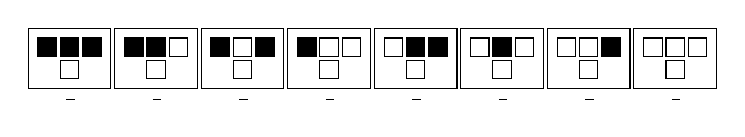
\begin{tikzpicture}[b/.style={draw, minimum size=2mm, fill=black},w/.style={draw, minimum size=2mm},m/.style={matrix of nodes, column sep=1pt, row sep=1pt, draw, label=below:#1}, node distance=1pt]
	          \matrix (A) [m=\_]{
	            |[b]|&|[b]|&|[b]|\\
	            &|[w]|\\
	          };
	          \matrix (B) [m=\_, right=of A]{
	            |[b]|&|[b]|&|[w]|\\
	            &|[w]|\\
	          };
	          \matrix (C) [m=\_, right=of B]{
	            |[b]|&|[w]|&|[b]|\\
	            &|[w]|\\
	          };
	          \matrix (D) [m=\_, right=of C]{
	            |[b]|&|[w]|&|[w]|\\
	            &|[w]|\\
	          };
	          \matrix (E) [m=\_, right=of D]{
	            |[w]|&|[b]|&|[b]|\\
	            &|[w]|\\
	          };
	          \matrix (F) [m=\_, right=of E]{
	            |[w]|&|[b]|&|[w]|\\
	            &|[w]|\\
	          };
	          \matrix (G) [m=\_, right=of F]{
	            |[w]|&|[w]|&|[b]|\\
	            &|[w]|\\
	          };
	          \matrix (H) [m=\_, right=of G]{
	            |[w]|&|[w]|&|[w]|\\
	            &|[w]|\\
	          };
	        \end{tikzpicture}
	      \end{center}
	    \end{minipage}
	    \ \\[27pt]
	    \begin{minipage}{0.25\textwidth}
	      Rule \#173
	    \end{minipage}
	    \begin{minipage}{0.75\textwidth}
	      \begin{center}
	        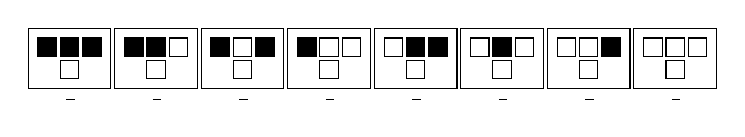
\begin{tikzpicture}[b/.style={draw, minimum size=2mm, fill=black},w/.style={draw, minimum size=2mm},m/.style={matrix of nodes, column sep=1pt, row sep=1pt, draw, label=below:#1}, node distance=1pt]
	          \matrix (A) [m=\_]{
	            |[b]|&|[b]|&|[b]|\\
	            &|[w]|\\
	          };
	          \matrix (B) [m=\_, right=of A]{
	            |[b]|&|[b]|&|[w]|\\
	            &|[w]|\\
	          };
	          \matrix (C) [m=\_, right=of B]{
	            |[b]|&|[w]|&|[b]|\\
	            &|[w]|\\
	          };
	          \matrix (D) [m=\_, right=of C]{
	            |[b]|&|[w]|&|[w]|\\
	            &|[w]|\\
	          };
	          \matrix (E) [m=\_, right=of D]{
	            |[w]|&|[b]|&|[b]|\\
	            &|[w]|\\
	          };
	          \matrix (F) [m=\_, right=of E]{
	            |[w]|&|[b]|&|[w]|\\
	            &|[w]|\\
	          };
	          \matrix (G) [m=\_, right=of F]{
	            |[w]|&|[w]|&|[b]|\\
	            &|[w]|\\
	          };
	          \matrix (H) [m=\_, right=of G]{
	            |[w]|&|[w]|&|[w]|\\
	            &|[w]|\\
	          };
	        \end{tikzpicture}
	      \end{center}
	    \end{minipage}
	    \ \\[36pt]
	    \QBlankBox{Shade in the appropriate boxes for each generation of the following ruleset.}
	    \begin{center}
	      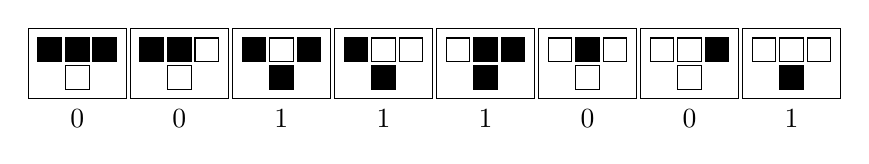
\begin{tikzpicture}[b/.style={draw, minimum size=3mm, fill=black},w/.style={draw, minimum size=3mm},m/.style={matrix of nodes, column sep=1pt, row sep=1pt, draw, label=below:#1}, node distance=1pt]
	        \matrix (A) [m=0]{
	          |[b]|&|[b]|&|[b]|\\
	          &|[w]|\\
	        };
	        \matrix (B) [m=0, right=of A]{
	          |[b]|&|[b]|&|[w]|\\
	          &|[w]|\\
	        };
	        \matrix (C) [m=1, right=of B]{
	          |[b]|&|[w]|&|[b]|\\
	          &|[b]|\\
	        };
	        \matrix (D) [m=1, right=of C]{
	          |[b]|&|[w]|&|[w]|\\
	          &|[b]|\\
	        };
	        \matrix (E) [m=1, right=of D]{
	          |[w]|&|[b]|&|[b]|\\
	          &|[b]|\\
	        };
	        \matrix (F) [m=0, right=of E]{
	          |[w]|&|[b]|&|[w]|\\
	          &|[w]|\\
	        };
	        \matrix (G) [m=0, right=of F]{
	          |[w]|&|[w]|&|[b]|\\
	          &|[w]|\\
	        };
	        \matrix (H) [m=1, right=of G]{
	          |[w]|&|[w]|&|[w]|\\
	          &|[b]|\\
	        };
	      \end{tikzpicture}
	    \end{center}

	    \begin{center}
	      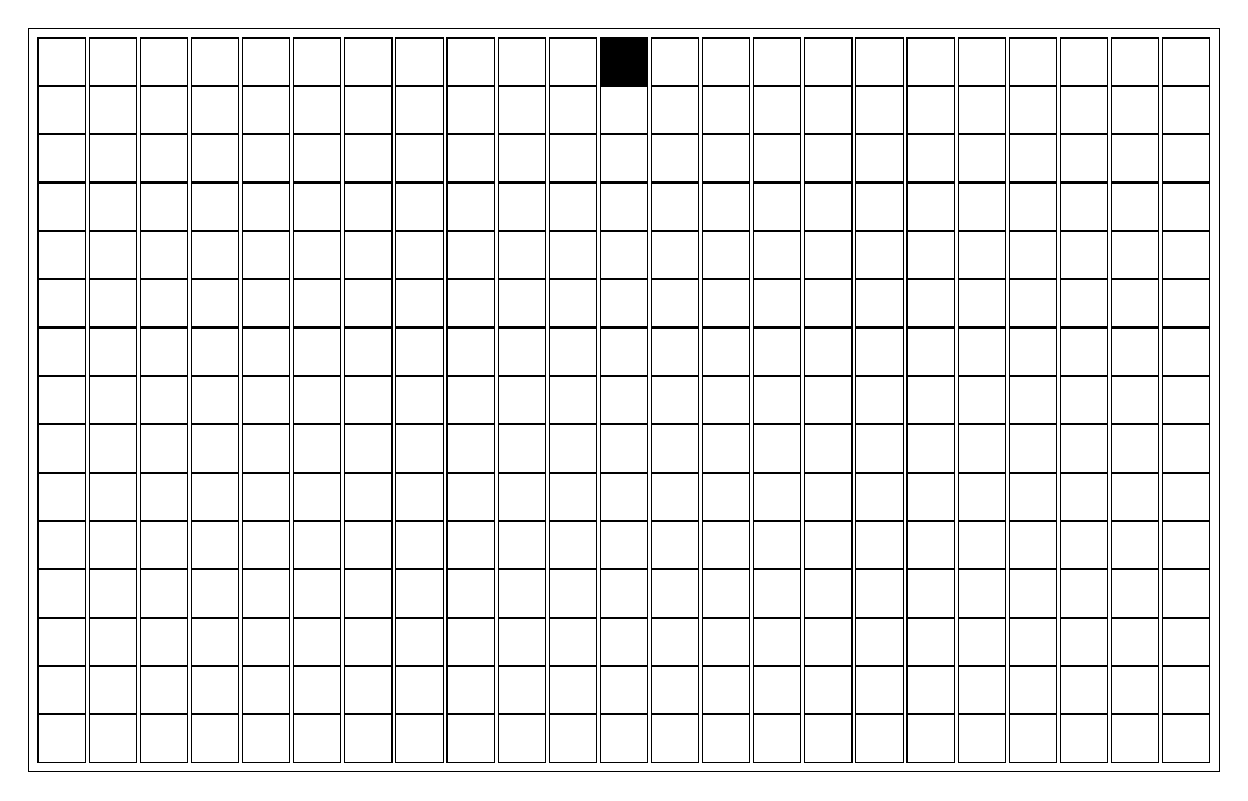
\begin{tikzpicture}[b/.style={draw, minimum size=6mm, fill=black},w/.style={draw, minimum size=6mm},m/.style={matrix of nodes, column sep=1pt, row sep=0pt, draw}, node distance=1pt]
	        \matrix [m]{
	           |[w]|&|[w]|&|[w]|&|[w]|&|[w]|&|[w]|&|[w]|&|[w]|&|[w]|&|[w]|&|[w]|&|[b]|&|[w]|&|[w]|&|[w]|&|[w]|&|[w]|&|[w]|&|[w]|&|[w]|&|[w]|&|[w]|&|[w]|\\
	           |[w]|&|[w]|&|[w]|&|[w]|&|[w]|&|[w]|&|[w]|&|[w]|&|[w]|&|[w]|&|[w]|&|[w]|&|[w]|&|[w]|&|[w]|&|[w]|&|[w]|&|[w]|&|[w]|&|[w]|&|[w]|&|[w]|&|[w]|\\
	           |[w]|&|[w]|&|[w]|&|[w]|&|[w]|&|[w]|&|[w]|&|[w]|&|[w]|&|[w]|&|[w]|&|[w]|&|[w]|&|[w]|&|[w]|&|[w]|&|[w]|&|[w]|&|[w]|&|[w]|&|[w]|&|[w]|&|[w]|\\
	           |[w]|&|[w]|&|[w]|&|[w]|&|[w]|&|[w]|&|[w]|&|[w]|&|[w]|&|[w]|&|[w]|&|[w]|&|[w]|&|[w]|&|[w]|&|[w]|&|[w]|&|[w]|&|[w]|&|[w]|&|[w]|&|[w]|&|[w]|\\
	           |[w]|&|[w]|&|[w]|&|[w]|&|[w]|&|[w]|&|[w]|&|[w]|&|[w]|&|[w]|&|[w]|&|[w]|&|[w]|&|[w]|&|[w]|&|[w]|&|[w]|&|[w]|&|[w]|&|[w]|&|[w]|&|[w]|&|[w]|\\
	           |[w]|&|[w]|&|[w]|&|[w]|&|[w]|&|[w]|&|[w]|&|[w]|&|[w]|&|[w]|&|[w]|&|[w]|&|[w]|&|[w]|&|[w]|&|[w]|&|[w]|&|[w]|&|[w]|&|[w]|&|[w]|&|[w]|&|[w]|\\
	           |[w]|&|[w]|&|[w]|&|[w]|&|[w]|&|[w]|&|[w]|&|[w]|&|[w]|&|[w]|&|[w]|&|[w]|&|[w]|&|[w]|&|[w]|&|[w]|&|[w]|&|[w]|&|[w]|&|[w]|&|[w]|&|[w]|&|[w]|\\
	           |[w]|&|[w]|&|[w]|&|[w]|&|[w]|&|[w]|&|[w]|&|[w]|&|[w]|&|[w]|&|[w]|&|[w]|&|[w]|&|[w]|&|[w]|&|[w]|&|[w]|&|[w]|&|[w]|&|[w]|&|[w]|&|[w]|&|[w]|\\
	           |[w]|&|[w]|&|[w]|&|[w]|&|[w]|&|[w]|&|[w]|&|[w]|&|[w]|&|[w]|&|[w]|&|[w]|&|[w]|&|[w]|&|[w]|&|[w]|&|[w]|&|[w]|&|[w]|&|[w]|&|[w]|&|[w]|&|[w]|\\
	           |[w]|&|[w]|&|[w]|&|[w]|&|[w]|&|[w]|&|[w]|&|[w]|&|[w]|&|[w]|&|[w]|&|[w]|&|[w]|&|[w]|&|[w]|&|[w]|&|[w]|&|[w]|&|[w]|&|[w]|&|[w]|&|[w]|&|[w]|\\
	           |[w]|&|[w]|&|[w]|&|[w]|&|[w]|&|[w]|&|[w]|&|[w]|&|[w]|&|[w]|&|[w]|&|[w]|&|[w]|&|[w]|&|[w]|&|[w]|&|[w]|&|[w]|&|[w]|&|[w]|&|[w]|&|[w]|&|[w]|\\
	           |[w]|&|[w]|&|[w]|&|[w]|&|[w]|&|[w]|&|[w]|&|[w]|&|[w]|&|[w]|&|[w]|&|[w]|&|[w]|&|[w]|&|[w]|&|[w]|&|[w]|&|[w]|&|[w]|&|[w]|&|[w]|&|[w]|&|[w]|\\
	           |[w]|&|[w]|&|[w]|&|[w]|&|[w]|&|[w]|&|[w]|&|[w]|&|[w]|&|[w]|&|[w]|&|[w]|&|[w]|&|[w]|&|[w]|&|[w]|&|[w]|&|[w]|&|[w]|&|[w]|&|[w]|&|[w]|&|[w]|\\
	           |[w]|&|[w]|&|[w]|&|[w]|&|[w]|&|[w]|&|[w]|&|[w]|&|[w]|&|[w]|&|[w]|&|[w]|&|[w]|&|[w]|&|[w]|&|[w]|&|[w]|&|[w]|&|[w]|&|[w]|&|[w]|&|[w]|&|[w]|\\
	           |[w]|&|[w]|&|[w]|&|[w]|&|[w]|&|[w]|&|[w]|&|[w]|&|[w]|&|[w]|&|[w]|&|[w]|&|[w]|&|[w]|&|[w]|&|[w]|&|[w]|&|[w]|&|[w]|&|[w]|&|[w]|&|[w]|&|[w]|\\
	        };
	      \end{tikzpicture}
	    \end{center}
    \QBox{What rule number is represented by the pattern in Question \#2?}{1cm}

  \pagebreak

	\section{Activity \#1}
		\subsection{Introduction}
	  In this activity, you will be implementing Wolfram's Classic Cellular Automation in Java. By creating the\\ \code{CellularAutomaton} class, you will be able to instantiate multiple \code{CellularAutomaton} objects in order to explore the various different cellular automata that could arise from different sets of rules. See the \emph{Template Class \& Test Cases} section for the skeletal outline of the \code{CellularAutomaton} class that you should use.

	  \subsection{Exercises}
	    \begin{enumerate}
	      \item Complete the \code{CellularAutomaton} class with the following specifications:
	        \begin{enumerate}
	          \item A constructor whose sole parameter is the size (number of array elements) of the automation. Default \code{rules} values should be set to Rule \#90 described in the background. The \code{cells} array should be initialized so that the middle cell is ``on''.
	          \item Two helper methods:
	          \begin{enumerate}
	            \item \code{getNeighbourValue} which returns the decimalisation of the binary configuration for a given cell and its neighbours.\\
							{\small\textbf{Note:} Remember to treat the ``edge cases'' differently. See the background for more information.}
	            \item \code{getNextGeneration} which evolves the automation according to its rules.
	          \end{enumerate}
	          \item One public method, \code{evolve}, which evolves the automation and prints the new generation to the console.
	        \end{enumerate}

	      \item Add the following to the \code{CellularAutomaton} class:
	        \begin{enumerate}
	          \item A helper method, \code{getRulePattern}, which takes a decimal \code{int} value and returns a set of rules corresponding to that value.
	          \item An overloaded constructor that allows the specification of a rule number to populate \code{rules} with.
	        \end{enumerate}
	    \end{enumerate}

    \subsection{Questions}
      \QBox{Briefly explain why the creation of the helper methods, \code{getNeighbourValue} and \code{getNextGeneration} may be desirable over placing all of the programming logic in the \code{evolve} method.}{4cm}
      \ \\[9pt]
      \QBox{Why should \code{getNextGeneration} return an array of cells representing the next generation rather than simply repopulating the \code{CellularAutomaton}'s \code{cells} array?}{4cm}

  \pagebreak

	\section{Activity \#2}
		\subsection{Introduction}
			In Stephen Wolfram's elementary cellular automata, the cells at the edge of a group (array index \code{0} and \code{length - 1}) assume the missing neighbour is `off' or $0$. In this activity, you will create a number of subclasses of your \code{CellularAutomaton} class to handle different behaviors for these special edge cases.

		\subsection{Exercises}
			\begin{enumerate}
				\item Create the \code{WrappingCellularAutomaton} subclass of \code{CellularAutomaton} in which edges ``wrap-around''. That is, the left-neighbour of cell \code{0} is actually at index \code{length - 1} and the right neighbour of cell \code{length - 1} is actually at index \code{0}.\\
				{\small\textbf{Note:} You will only receive full credit for this exercise if you take full advantage of inheritance through subclassing.}
				\item Create the \code{SpecialCaseCellularAutomaton} subclass of \code{CellularAutomaton} in which edges are given a special set of rules to handle only having two neighbours. You should implement a constructor that will accept two rule numbers, one for the main set of rules and one for the special edge cases.\\
				{\small\textbf{Note:} Because there are only two neighbours for these special edge cases, you will only need to store a total of $4$ different cases, with a maximum rule number of $16$.}
			\end{enumerate}

		\subsection{Questions}
			\QBox{How are the patterns that emerge from the \code{WrappingCellularAutomaton} different from those of the base \code{CellularAutomaton} for the same rule number? How are they similar?}{4cm}
			\ \\[9pt]
			\QBox{What base pattern did you choose for the four possibilities of edge cases in \code{SpecialCaseCellularAutomaton}? What led you to choose this pattern?}{4cm}

	\pagebreak

	\section{Final Analysis}
		\QBox{Find two sets of cellular automata rules that result in the same pattern. Explain why this occurs.}{3cm}
	  \ \\[9pt]
	  \QBox{Experiment with changing the pattern for Generation $0$ in your \code{CellularAutomaton} class. How does the starting pattern affect the overall pattern of the cellular automata.}{3cm}
	  \ \\[9pt]
	  \QBox{Which part of implementing \code{CellularAutomaton} did you find most challenging? How did you overcome these challenges?}{3cm}
	  \ \\[9pt]
	  \QBox{Which part of implementing \code{WrappingCellularAutomaton} or \code{SpecialCaseCellularAutomaton} did you find most challenging? How did you overcome these challenges?}{3cm}
	  \ \\[9pt]
	  \QBox{What new programming techniques or knowledge did you learn as a result of this lab?}{3cm}

  \pagebreak
  \blankpage
  \pagebreak

	\section{Template Class \& Test Cases}
		\lstinputlisting[basicstyle=\small\ttfamily,tabsize=2]{files/CellularAutomata.java}
\end{document}
